% !TEX program = xelatex
\documentclass[12pt,a4paper,fontset=fandol]{ctexart}
\usepackage[left=22mm,right=22mm,top=22mm,bottom=22mm]{geometry}
\usepackage{amsmath,amssymb,bm,mathtools}
\usepackage{graphicx,xcolor,booktabs,longtable,array}
\usepackage{tikz}
\usetikzlibrary{arrows.meta,calc,decorations.pathmorphing}
\usepackage{setspace,enumitem,fancyhdr}
\usepackage[unicode,hidelinks]{hyperref}
\setstretch{1.24}
\setlength{\parindent}{2em}
\setlength{\parskip}{.35em}
\setlength{\emergencystretch}{2em}
\setlist{nosep,leftmargin=2em}
\setcounter{secnumdepth}{-1}
\ctexset{section={format=\Large\bfseries,beforeskip=1em,afterskip=.7em},
subsection={format=\large\bfseries,beforeskip=.8em,afterskip=.4em},
subsubsection={format=\normalsize\bfseries,beforeskip=.7em,afterskip=.3em}}
\allowdisplaybreaks[2]
\tikzset{arr/.style={-{Stealth[length=2mm]},semithick},
dot/.style={circle,fill,inner sep=1.5pt}}
\providecommand{\tightlist}{\setlength{\itemsep}{0pt}\setlength{\parskip}{0pt}}
\providecommand{\pandocbounded}[1]{#1}
\newsavebox{\diagrambox}
\pagestyle{fancy}
\fancyhf{}
\renewcommand{\headrulewidth}{0pt}
\fancyfoot[C]{\small \thepage}
\setlength{\headheight}{16pt}
\begin{document}
\begin{titlepage}
\thispagestyle{empty}
\vspace*{27mm}
\begin{center}
{\LARGE\bfseries 第42届全国中学生物理竞赛\par}
\vspace{8mm}
{\LARGE\bfseries 复赛理论试题\par}
\vspace{17mm}
{\Large 试题版\par}
\end{center}
\vfill
\end{titlepage}
\setcounter{page}{1}
本卷共7题，总分320分。考试时间：9:00---12:00。所有需要评阅的解答均须写在答题纸上。

\section{第 1
题　冷原子云的自由展开与飞行时间测温}\label{ux7b2c-1-ux9898-ux51b7ux539fux5b50ux4e91ux7684ux81eaux7531ux5c55ux5f00ux4e0eux98deux884cux65f6ux95f4ux6d4bux6e29}

一磁光陷阱中约束的 \(N\) 个原子构成的原子气处于绝对温度 \(T\)
的平衡态。在位置 \(\mathbf r=(x,y,z)\)、速度 \(\mathbf v=(v_x,v_y,v_z)\)
的原子数密度 \(f(\mathbf r,\mathbf v)\) 服从玻尔兹曼分布 \[
f(\mathbf r,\mathbf v)\propto
\exp\!\left[-\frac{m(\omega_x^2x^2+\omega_y^2y^2+\omega_z^2z^2)}{2k_{\rm B}T}\right]
\exp\!\left[-\frac{m(v_x^2+v_y^2+v_z^2)}{2k_{\rm B}T}\right].
\] 其中 \(\omega_i\) 为 \(i=x,y,z\) 方向陷阱对原子的约束强度，\(m\)
为原子质量，\(k_{\rm B}\) 为玻尔兹曼常量。取竖直向下为 \(z\)
轴正方向。在陷阱正下方 \(z=h\)（\(h>0\)）处有探测器，可测量该平面附近沿
\(z\)
方向单位高度内的原子数，以及单位时间内由上至下通过该平面的原子数。重力加速度大小为
\(g\)，忽略原子碰撞，\(t=0\) 时撤除陷阱。

（1）求撤除前完整的分布函数 \(f(\mathbf r,\mathbf v)\)。

（2）求 \(t>0\) 时探测平面附近的纵向数密度 \(n(t)\) 和通过该平面的原子流
\(I(t)\)。

（3）在温度极低、约束很强的极限下，求 \(n(t)\) 最大时刻 \(t_n\) 和
\(I(t)\) 最大时刻 \(t_I\)，保留温度的非零最低阶。

（4）在同一极限下，\(t=t_n\) 附近有 \[
n(t)\approx n_0\exp\!\left[-\frac{(t-t_n)^2}{2\sigma_t^2}\right].
\] 求有效展宽 \(\sigma_t\)，保留温度的非零最低阶。提示：
\(\int_0^\infty e^{-x^2}\,dx=\sqrt\pi/2\)，
\(\int_0^\infty x^2e^{-x^2}\,dx=\sqrt\pi/4\)。本题45分。

\begin{center}
\begin{minipage}{\linewidth}
\centering\begingroup
\sbox{\diagrambox}{\small
\begin{tikzpicture}[scale=.85]
\draw[->](-2,0)--(2.2,0)node[right]{$x$};
\draw[->](0,1.6)--(0,-2.7)node[below]{$z$};
\draw[blue,thick] plot[domain=-1.5:1.5,samples=60](\x,{.65*\x*\x+.3});
\foreach \x/\y in {-.7/.15,-.2/.4,.3/.1,.65/.32,.12/-.15,-.4/-.12}
 \fill[blue](\x,\y)circle(2pt);
\node[left] at(-.9,.65){原子云};
\draw[dashed](-1.8,-2)--(1.8,-2)node[right]{$z=h$};
\draw[fill=gray!20](-1.5,-2.2)rectangle(1.5,-2);
\node[below] at(0,-2.2){探测平面};
\draw[->,thick](1,-.4)--(1,-1.4)node[midway,right]{$g$};
\node[above right] at(0,0){$O$};
\end{tikzpicture}
}
\ifdim\wd\diagrambox>.88\linewidth
\sbox{\diagrambox}{\resizebox{.88\linewidth}{!}{\usebox{\diagrambox}}}
\fi
\ifdim\ht\diagrambox>.40\textheight
\resizebox{!}{.40\textheight}{\usebox{\diagrambox}}
\else\usebox{\diagrambox}\fi
\par\smallskip{\small 图1-1　竖直向下为正，陷阱撤除后原子云展开并落向探测平面。\par}
\endgroup\end{minipage}
\end{center}

\clearpage

\section{第 2
题　重离子束探针与平行板能量分析器}\label{ux7b2c-2-ux9898-ux91cdux79bbux5b50ux675fux63a2ux9488ux4e0eux5e73ux884cux677fux80fdux91cfux5206ux6790ux5668}

重离子束探针通过二次离子的能量测量等离子体局部电势。一次离子电荷量
\(q_1=e\)（\(e>0\)），初始动能为 \(K_1\)；在等离子体内直接电离成电荷量
\(q_2=2e\)
的二次离子。二次离子在外部磁场偏转下离开等离子体，恰能进入能量分析器，其进入狭缝的动能为
\(K_2\)。等离子体外电势为零，相对论效应可忽略。

\begin{center}
\begin{minipage}{\linewidth}
\centering\begingroup
\sbox{\diagrambox}{\small
\scalebox{.80}{\begin{tikzpicture}[scale=.9]
\fill[gray!15](0,0)circle(1.45);
\node at(0,-.75){等离子体 $\Phi$};
\draw[->,thick](-3,1.4)--(-.4,.4)node[midway,above=7pt,fill=white,inner sep=2pt]{一次离子 $q_1,K_1$};
\fill(-.4,.4)circle(2pt);
\draw[->,thick](-.4,.4)--(3,1.1)node[midway,above=7pt,fill=white,inner sep=2pt]{二次离子 $q_2$};
\draw[very thick](3,.4)--(3.2,1.6);
\node[right]at(3.2,1){能量分析器 $K_2$};
\node[below]at(-.4,.4){测量位置};
\node at(.6,-.1){$\otimes\,B$};
\end{tikzpicture}
}
}
\ifdim\wd\diagrambox>.88\linewidth
\sbox{\diagrambox}{\resizebox{.88\linewidth}{!}{\usebox{\diagrambox}}}
\fi
\ifdim\ht\diagrambox>.40\textheight
\resizebox{!}{.40\textheight}{\usebox{\diagrambox}}
\else\usebox{\diagrambox}\fi
\par\smallskip{\small 图2-1　二次离子从测量位置离开等离子体，分析器测量其末动能。\par}
\endgroup\end{minipage}
\end{center}

能量分析器由相距 \(d\) 的两平行电极板组成，上板电势
\(V_A\)，下板电势0；只有两板之间存在均匀电场，其他区域无电场、磁场。二次离子速度平行于纸面。入射狭缝中心在下板下方
\(Y_{D1}\)，接收中心在下板下方 \(Y_{D2}\)。相对水平板的入射角为
\(\theta_I\)，接收时相对入射中心的水平距离为 \(X_D\)。

\begin{center}
\begin{minipage}{\linewidth}
\centering\begingroup
\sbox{\diagrambox}{\small
\scalebox{.80}{\begin{tikzpicture}[scale=.85]
\draw[very thick](-1,2)--(6,2)node[right]{$V_A$};
\draw[very thick](-1,.8)--(.3,.8);
\draw[very thick](1,.8)--(3.7,.8);
\draw[very thick](4.4,.8)--(6,.8)node[right]{$V=0$};
\draw[<->](-1.3,.8)--(-1.3,2)node[midway,left]{$d$};
\draw[blue,thick](0,-.5)--(.7,.8);
\draw[blue,thick] plot[domain=.7:4.1,samples=50](\x,{.8+1.1*(1-((\x-2.4)/1.7)^2)});
\draw[blue,thick](4.1,.8)--(4.8,-.5);
\draw[very thick](-.5,.3)--(.5,-1.3);
\draw[very thick](4.3,-1.3)--(5.3,.3);
\draw[<->](0,-1.65)--(4.8,-1.65)node[midway,below]{$X_D$};
\draw[dashed](0,-.5)--(4.8,-.5);
\draw[<->](.1,-.5)--(.1,.8)node[midway,left]{$Y_{D1}$};
\draw[<->](4.9,-.5)--(4.9,.8)node[midway,right]{$Y_{D2}$};
\draw[blue] (.42,-.5) arc(0:62:.42);\node[blue]at(.55,-.2){$\theta_I$};
\draw(.65,-.5) arc(0:-58:.65);\node[right]at(.6,-.92){$\theta_a$};
\draw(4.15,-.5) arc(180:238:.65);\node[left]at(4.2,-.92){$\theta_b$};
\draw[->] (0,-.5)--(.5,-1.3);\draw[->] (4.8,-.5)--(4.3,-1.3);
\node at(-.45,-.75){$l$}; \node at(5.15,-.8){$s$};
\node at(2.5,2.4){电场向下；图中高度与角度为示意};
\end{tikzpicture}
}
}
\ifdim\wd\diagrambox>.88\linewidth
\sbox{\diagrambox}{\resizebox{.88\linewidth}{!}{\usebox{\diagrambox}}}
\fi
\ifdim\ht\diagrambox>.40\textheight
\resizebox{!}{.40\textheight}{\usebox{\diagrambox}}
\else\usebox{\diagrambox}\fi
\par\smallskip{\small 图2-2　平行板内轨迹为抛物线，板外为直线；入口与出口处轨迹斜率相反。\par}
\endgroup\end{minipage}
\end{center}

（1.1）求 \(X_D\)。 （1.2）要求 \(\theta_I\) 的极小变化
\(\Delta\theta_I\) 使 \(X_D\) 的变化为
\(O((\Delta\theta_I)^3)\)，即满足二级聚焦。求 \(0<\theta_I<\pi/2\)
内的聚焦角，并给出 \(X_D,V_A\)。
（1.3）分析器已按上述条件放置，入射板、接收板与水平方向夹角分别为
\(\theta_a,\theta_b\)。离子在入射板上距狭缝中心为
\(l\)（沿板向右下方为正），求接收板上距中心的 \(s\)；\(s>0\)
为下半平面，\(s<0\) 为上半平面。

（2）安装误差和 \(K_2\) 波动可能使分析器偏离二级聚焦，入射狭缝宽为
\(w\)。 （2.1）求 \(l=0\) 时的 \(s\)。
（2.2）假设入射离子全部被捕获，且狭缝各处入射的离子密度、动能、速度方向相同。上、下半平面接收电流分别为
\(i_U,i_L\)，用这些电流及硬件参数表示 \(K_2\)。
（2.3）测量位置处的直接电离可简化为 \[
\mathrm{Tl}^+(\text{极高能})+e^-(\text{低能})
\longrightarrow \mathrm{Tl}^+(\text{极高能})+e^-(\text{次级高能})
\] \[
\longrightarrow
\mathrm{Tl}^{++}(\text{极高能})+e'^-(\text{次级高能})+e''^-(\text{逸出}).
\]
次级高能电子使一次离子电离；电子动能和电离能远小于一次离子动能，没有其他碰撞。忽略离子从出发至测量位置、以及二次离子从测量位置至分析器期间的能量衰减，求局部电势
\(\Phi\)。本题45分。

\clearpage

\section{第 3
题　量子霍尔电阻的接触误差与多重连接}\label{ux7b2c-3-ux9898-ux91cfux5b50ux970dux5c14ux7535ux963bux7684ux63a5ux89e6ux8befux5deeux4e0eux591aux91cdux8fdeux63a5}

量子霍尔效应器件的端口按图标记为1至8，垂直器件向上施加磁场
\(B\)。在不相邻的端口 \(i,j\) 通电流 \(I_0\)，在连接 \(i,j\)
的直线段两侧各选端口 \(l,m\) 测电压 \(U_{lm}\)，定义霍尔电阻 \[
R_{i,j;l,m}=\frac{U_{lm}}{I_0}.
\]

\begin{center}
\begin{minipage}{\linewidth}
\centering\begingroup
\sbox{\diagrambox}{\small
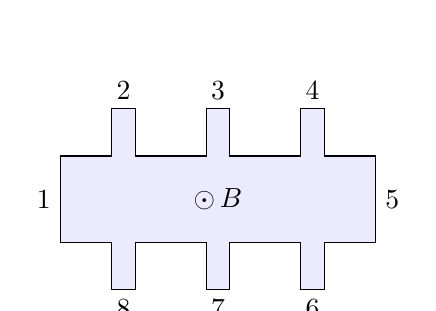
\begin{tikzpicture}
\draw[fill=blue!8](-2,-.55)--(-1.35,-.55)--(-1.35,-1.15)--(-1.05,-1.15)--(-1.05,-.55)--(-.15,-.55)--(-.15,-1.15)--(.15,-1.15)--(.15,-.55)--(1.05,-.55)--(1.05,-1.15)--(1.35,-1.15)--(1.35,-.55)--(2,-.55)--(2,.55)--(1.35,.55)--(1.35,1.15)--(1.05,1.15)--(1.05,.55)--(.15,.55)--(.15,1.15)--(-.15,1.15)--(-.15,.55)--(-1.05,.55)--(-1.05,1.15)--(-1.35,1.15)--(-1.35,.55)--(-2,.55)--cycle;
\node[left]at(-2,0){1};\node[right]at(2,0){5};
\foreach \x/\n in {-1.2/2,0/3,1.2/4}\node[above]at(\x,1.15){\n};
\foreach \x/\n in {-1.2/8,0/7,1.2/6}\node[below]at(\x,-1.15){\n};
\node at(0,0){$\odot\,B$};
\end{tikzpicture}
}
\ifdim\wd\diagrambox>.88\linewidth
\sbox{\diagrambox}{\resizebox{.88\linewidth}{!}{\usebox{\diagrambox}}}
\fi
\ifdim\ht\diagrambox>.40\textheight
\resizebox{!}{.40\textheight}{\usebox{\diagrambox}}
\else\usebox{\diagrambox}\fi
\par\smallskip{\small 图3-1　八端口器件的端口编号与垂直磁场。\par}
\endgroup\end{minipage}
\end{center}

器件等效为含受控电源的环形电路。流入端口 \(i\) 的电流为
\(I_i\)，流出时取负；每端口固有电阻为 \(r=R_{\rm H}/2\)，外加接触电阻
\(R_{ci}\)。相邻内部节点间的电源电动势为
\(r(I_i+I_{i+1})\)，电源无内阻，方向与图示磁场约定一致。各接触电阻可不同，但
\(\epsilon_i=R_{ci}/r\) 均为远小于1的量，约 \(0.1\%\)。

\begin{center}
\begin{minipage}{\linewidth}
\centering\begingroup
\sbox{\diagrambox}{\small
\begin{tikzpicture}[scale=.85]
\foreach \i/\a in {1/180,2/135,3/90,4/45,5/0,6/-45,7/-90,8/-135}{
 \coordinate (p\i) at(\a:2.6);
 \coordinate (t\i) at(\a:4.3);
 \draw (p\i)--(t\i);
 \node[draw,fill=white,inner sep=2pt]at(\a:3.12){$r$};
 \node[draw,fill=white,inner sep=2pt]at(\a:3.72){$R_{c\number\i}$};
 \node at(\a:4.68){$\number\i$};
 \fill(p\i)circle(1.5pt);
}
\foreach \i/\j in {1/2,2/3,3/4,4/5,5/6,6/7,7/8,8/1}{
 \draw[->] (p\i)--node[fill=white,inner sep=1pt]{$E_{\number\i,\number\j}$}(p\j);
}
\node[font=\small] at(0,.45){受控电源环};
\node[font=\scriptsize] at(0,-.05){$E_{ij}=r(I_i+I_j)$};
\node[font=\scriptsize] at(0,-.55){$C_{i+1}-C_i=E_{i,i+1}$};
\end{tikzpicture}
}
\ifdim\wd\diagrambox>.88\linewidth
\sbox{\diagrambox}{\resizebox{.88\linewidth}{!}{\usebox{\diagrambox}}}
\fi
\ifdim\ht\diagrambox>.40\textheight
\resizebox{!}{.40\textheight}{\usebox{\diagrambox}}
\else\usebox{\diagrambox}\fi
\par\smallskip{\small 图3-2　八个受控电源及端口串联电阻；箭头方向表示内部节点电势升高方向，指标按模8循环。\par}
\endgroup\end{minipage}
\end{center}

（1）哪些端口通电流、哪些端口测电压，可以获得与接触电阻无关的霍尔电阻？至少证明一种接法。

（2）将两个性质相同、接触电阻可能不同的器件 \(a,b\) 相连，端口记为
\(1a\) 至 \(8a\)、\(1b\) 至 \(8b\)。 （2.1）按图3-3相连，求 \(7a\) 与
\(3b\) 断开和接通时，在 \(1a,5b\) 通电流、\(3a,7b\) 测电压的霍尔电阻
\(R_{1a,5b;3a,7b}\) 及
\(R'_{1a,5b;3a,7b}\)。哪种接法的相对接触误差更小？证明结论。

\begin{center}
\begin{minipage}{\linewidth}
\centering\begingroup
\sbox{\diagrambox}{\small
\begin{tikzpicture}
\foreach \x/\s in {0/a,5/b}{
 \draw[fill=blue!8](\x-1,-.7)rectangle(\x+1,.7);
 \node at(\x,0){器件 $\s$};
 \foreach \dx/\dy/\n in {-1/0/1,1/0/5,0/.7/3,0/-.7/7}{
  \coordinate(\s\n)at(\x+\dx,\dy);
  \node at(\x+\dx*1.25,\dy*1.4){$\n\s$};
 }
}
\draw[->](-2.3,0)--(a1)node[midway,above]{$I$};
\draw(a5)--(b1);\node[above]at(1.8,.08){主连接};
\draw[->](b5)--(7.3,0)node[midway,above]{$I$};
\draw(a7)--(0,-1.6)--(2.7,-1.6)--(2.7,-.18) to[out=0,in=0](2.7,.18)--(2.7,1.6)--(5,1.6)--(b3);
\node[below]at(1.5,-1.6){可断开的补偿连接};
\draw(a3)--(0,1.6)node[above]{$U_{3a}$};
\draw(b7)--(5,-1.6)node[below]{$U_{7b}$};
\end{tikzpicture}
}
\ifdim\wd\diagrambox>.88\linewidth
\sbox{\diagrambox}{\resizebox{.88\linewidth}{!}{\usebox{\diagrambox}}}
\fi
\ifdim\ht\diagrambox>.40\textheight
\resizebox{!}{.40\textheight}{\usebox{\diagrambox}}
\else\usebox{\diagrambox}\fi
\par\smallskip{\small 图3-3　主连接为5a与1b；补偿连接为7a与3b，测量端口为3a与7b。\par}
\endgroup\end{minipage}
\end{center}

（2.2）三重并联接法为：\(1a,1b\) 接输入 \(A\)，\(5a,5b\) 接输出
\(B\)；\(2a,2b\) 相连但不外接；\(3a,3b\) 相连并接电压端 \(C\)；\(6a,6b\)
相连但不外接；\(7a,7b\) 相连并接电压端 \(D\)。求 \(R_{A,B;C,D}\)
的接触电阻相对误差阶。假设
\(R_{c5a}=R_{c5b}=R_{c6a}=R_{c6b}=R_{c7a}=R_{c7b}=0\)，证明结论。本题45分。

\begin{center}
\begin{minipage}{\linewidth}
\centering\begingroup
\sbox{\diagrambox}{\small
\begin{tikzpicture}[scale=.8]
\draw[fill=blue!8](-3,-3)rectangle(-1,3);
\draw[fill=blue!8](1,-3)rectangle(3,3);
\node at(-2,0){$a$};\node at(2,0){$b$};
\foreach \y/\i in {2.2/2,1/3,-1/6,-2.2/7}{
 \draw(-1,\y)--(1,\y);
 \node[left,fill=blue!8,inner sep=1pt]at(-1,\y){$\i a$};
 \node[right,fill=blue!8,inner sep=1pt]at(1,\y){$\i b$};
}
\draw(-3,0)--(-3.8,0)--(-3.8,3.7)--(3.8,3.7)--(3.8,0)--(3,0);
\node[above]at(0,3.7){$A:\ 1a,1b$};
\draw(-2,-3)--(-2,-3.8)--(2,-3.8)--(2,-3);
\node[below]at(0,-3.8){$B:\ 5a,5b$};
\node[above,font=\small]at(0,2.2){浮置连接};
\node[above]at(0,1){$C:\ 3a,3b$};
\node[above,font=\small]at(0,-1){浮置连接};
\node[above]at(0,-2.2){$D:\ 7a,7b$};
\end{tikzpicture}
}
\ifdim\wd\diagrambox>.88\linewidth
\sbox{\diagrambox}{\resizebox{.88\linewidth}{!}{\usebox{\diagrambox}}}
\fi
\ifdim\ht\diagrambox>.40\textheight
\resizebox{!}{.40\textheight}{\usebox{\diagrambox}}
\else\usebox{\diagrambox}\fi
\par\smallskip{\small 图3-4　三重并联的连接清单；交叉线以端口名称判定，C与D均为高阻测量端。\par}
\endgroup\end{minipage}
\end{center}

\clearpage

\section{第 4
题　强平面激光场中的相对论电子运动}\label{ux7b2c-4-ux9898-ux5f3aux5e73ux9762ux6fc0ux5149ux573aux4e2dux7684ux76f8ux5bf9ux8bbaux7535ux5b50ux8fd0ux52a8}

真空激光加速机制利用强激光脉冲提高电子能量。采用沿 \(+z\)
传播、线偏振的单色平面电磁波模型： \[
\mathbf E=E_0\cos(kz-\omega t)\,\mathbf e_x,\qquad
\mathbf B=\frac{E_0}{c}\cos(kz-\omega t)\,\mathbf e_y,
\qquad kc=\omega.
\] \(E_0\) 是电场振幅，\(c\) 为真空光速。忽略重力，使用相对论动力学。

（1）\(t=0\) 时电子静止于原点，忽略辐射阻尼。 （1.1）求动量
\(\mathbf p\) 和总能量 \(\varepsilon\)，表达式可含当时坐标。
（1.2）求位置 \(x,y,z\) 与时间的关系，可用隐函数表示。

（2）\(t=0\) 时从原点沿 \(x\)-\(z\) 平面注入总能量为 \(\varepsilon_0\)
的电子，初速度与 \(+x\) 的夹角不大于 \(\pi/2\)，忽略辐射阻尼。求最大能量
\(\varepsilon_{\max}\) 及对应入射角 \(\theta_0\)；\(\theta_0\)
为入射方向与 \(z\) 轴的夹角。

（3）强激光下辐射阻尼不可忽略，给定能量损失模型 \[
\frac{d\varepsilon}{dt}
=-\frac{e^4\mu_0E_0^2}{4\pi m_e^4c^5}\varepsilon^2.
\] 激光强度 \(I=1.0\times10^{22}\,\mathrm{W/cm^2}\)，波长
\(\lambda=800\,\mathrm{nm}\)，初始总能量
\(\varepsilon_0=1000m_ec^2\)。求一个激光周期后
\(\Delta\varepsilon/\varepsilon_0\)。 给定
\(m_e=9.101\times10^{-31}\,\mathrm{kg}\)，
\(e=1.602\times10^{-19}\,\mathrm C\)，
\(c=2.998\times10^8\,\mathrm{m/s}\)，
\(\mu_0=4\pi\times10^{-7}\,\mathrm{N/A^2}\)。
强度为坡印廷矢量大小的时间平均。本题50分。

\begin{center}
\begin{minipage}{\linewidth}
\centering\begingroup
\sbox{\diagrambox}{\small
\begin{tikzpicture}
\draw[->](0,0)--(5,0)node[right]{$z$};
\draw[->](1,0)--(1,1.7)node[above]{$E_x$};
\draw[->](1,0)--(.1,-.8)node[left]{$B_y$};
\draw[blue,thick]plot[domain=0:4.6,samples=100](\x,{.75*cos(180*\x)});
\node at(3,1.5){$\mathbf E\times\mathbf B\parallel+\hat{\mathbf z}$};
\node[below]at(3,-1){电子电荷 $-e$，受力为 $-e(\mathbf E+\mathbf v\times\mathbf B)$};
\end{tikzpicture}
}
\ifdim\wd\diagrambox>.88\linewidth
\sbox{\diagrambox}{\resizebox{.88\linewidth}{!}{\usebox{\diagrambox}}}
\fi
\ifdim\ht\diagrambox>.40\textheight
\resizebox{!}{.40\textheight}{\usebox{\diagrambox}}
\else\usebox{\diagrambox}\fi
\par\smallskip{\small 图4-1　电场、磁场与传播方向相互垂直；电子电荷为负。\par}
\endgroup\end{minipage}
\end{center}

\clearpage

\section{第 5
题　约瑟夫森结的时间相位、磁通干涉与小振动}\label{ux7b2c-5-ux9898-ux7ea6ux745fux592bux68eeux7ed3ux7684ux65f6ux95f4ux76f8ux4f4dux78c1ux901aux5e72ux6d89ux4e0eux5c0fux632fux52a8}

理想约瑟夫森结由``超导体---薄绝缘层---超导体''组成。以结中心为原点，绝缘层厚度为
\(d\ll Y,Z\)，其 \(y\)-\(z\) 截面的边长为 \(Y,Z\)；电流沿 \(x\)
方向。两超导体波函数相位分别为 \(\varphi_1,\varphi_2\)，相位差
\(\delta=\varphi_2-\varphi_1\)。结电流密度和相位满足 \[
j=j_0\sin\delta,\qquad
\frac{\partial\delta}{\partial t}=\frac{2e}{\hbar}U.
\] \(j_0>0\)，\(\hbar\)
为约化普朗克常量，\(e>0\)。以上关系在外磁场为零和非零时均成立；无外磁场时相位差与空间无关。

\begin{center}
\begin{minipage}{\linewidth}
\centering\begingroup
\sbox{\diagrambox}{\small
\begin{tikzpicture}
\draw[fill=blue!12](-2,-1.5)rectangle(-.3,1.5);
\draw[fill=gray!40](-.3,-1.5)rectangle(.3,1.5);
\draw[fill=blue!12](.3,-1.5)rectangle(2,1.5);
\node at(-1.25,1){超导体1};\node at(1.25,1){超导体2};
\draw[dashed](-.7,-1.5)--(-.7,1.5);\draw[dashed](.7,-1.5)--(.7,1.5);
\draw[<->](-.7,-1.9)--(.7,-1.9)node[midway,below]{$d+2\lambda$};
\draw[->](-2.8,0)--(2.8,0)node[right]{$x$};
\draw[->](0,-1.5)--(0,2.2)node[above]{$y$};
\node[fill=white,inner sep=2pt] at(0,.15){$\odot B_z$};
\node at(-1.2,-.8){$\varphi_1$};\node at(1.2,-.8){$\varphi_2$};
\end{tikzpicture}
}
\ifdim\wd\diagrambox>.88\linewidth
\sbox{\diagrambox}{\resizebox{.88\linewidth}{!}{\usebox{\diagrambox}}}
\fi
\ifdim\ht\diagrambox>.40\textheight
\resizebox{!}{.40\textheight}{\usebox{\diagrambox}}
\else\usebox{\diagrambox}\fi
\par\smallskip{\small 图5-1　绝缘层与两侧磁场穿透区域形成有效磁厚度 $d+2\lambda$。\par}
\endgroup\end{minipage}
\end{center}

（1）结两端加恒定直流电压 \(U_0\)，初相位为 \(\delta(0)\)。求电流密度
\(j(t)\) 及周期。

（2）令 \(U=0\)，沿 \(z\)
方向加静磁场。由于超导体屏蔽，磁场只存在于绝缘层及两侧各厚度为
\(\lambda\) 的等效区域。绝缘层内
\(\mathbf B=B_z(y)\mathbf e_z\)，相位满足 \[
\frac{d\delta}{dy}=\frac{2e(d+2\lambda)}{\hbar}B_z(y).
\] （2.1）忽略电流自生磁场，\(B_z=B_0\) 为常数。求 \(\delta(y)\)、总电流
\(I_J(B_0)\)，以及 \(I_J=0\) 对应的 \(B_0\)。已知
\(\delta(0)=\delta_0\ne k\pi\)。 （2.2）考虑电流自生磁场，证明 \[
\frac{d^2\delta}{dy^2}=\frac1{\lambda_J^2}\sin\delta,
\] 并求约瑟夫森穿透深度 \(\lambda_J\)。绝缘层磁导率为 \(\mu_0\)。

（3）外磁场为零，宏观模型为理想约瑟夫森结 \(J\) 与电阻 \(R\)、电容 \(C\)
并联，外加恒定偏置电流 \(I\)，记 \(I_0=j_0YZ\)。

\begin{center}
\begin{minipage}{\linewidth}
\centering\begingroup
\sbox{\diagrambox}{\small
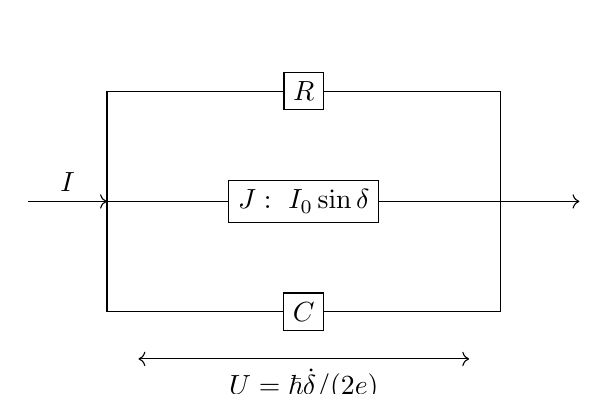
\begin{tikzpicture}
\coordinate(A)at(0,0);\coordinate(B)at(5,0);
\draw[->](-1,0)--(A)node[midway,above]{$I$};
\draw(A)--(0,1.4)--(5,1.4)--(B);
\node[draw,fill=white]at(2.5,1.4){$R$};
\draw(A)--(B); \node[draw,fill=white]at(2.5,0){$J:\ I_0\sin\delta$};
\draw(A)--(0,-1.4)--(5,-1.4)--(B);
\node[draw,fill=white]at(2.5,-1.4){$C$};
\draw[->](B)--(6,0);
\draw[<->](.4,-2)--(4.6,-2)node[midway,below]{$U=\hbar\dot\delta/(2e)$};
\end{tikzpicture}
}
\ifdim\wd\diagrambox>.88\linewidth
\sbox{\diagrambox}{\resizebox{.88\linewidth}{!}{\usebox{\diagrambox}}}
\fi
\ifdim\ht\diagrambox>.40\textheight
\resizebox{!}{.40\textheight}{\usebox{\diagrambox}}
\else\usebox{\diagrambox}\fi
\par\smallskip{\small 图5-2　电阻、电容与理想约瑟夫森结并联，三个支路具有相同电压。\par}
\endgroup\end{minipage}
\end{center}

（3.1）用 \(\delta(t)\) 及其导数表示三个支路电流，导出相位方程。
以下认为 \(R\) 足够大，可忽略电阻支路。
（3.2）将方程类比为单位质量粒子在势 \(V(\delta)\)
中运动。求势、存在势阱的电流范围、阱底相位及小振动角频率 \(\omega\)。
（3.3）\(\omega\) 的最大值为 \(\omega_J\)，已知结中电磁波速度
\(\tilde c=\omega_J\lambda_J\)。绝缘层相对介电常数
\(\epsilon_r=9.0\)，\(d=3.0\,\mathrm{nm}\)，\(\lambda=53\,\mathrm{nm}\)，求
\(\tilde c/c\)，保留两位有效数字。本题45分。

\clearpage

\section{第 6
题　转速仪的定倾角运动、冲击与进动速率}\label{ux7b2c-6-ux9898-ux8f6cux901fux4eeaux7684ux5b9aux503eux89d2ux8fd0ux52a8ux51b2ux51fbux4e0eux8fdbux52a8ux901fux7387}

竖直转轴底端由光滑地面支撑，受固定光滑轴承 \(A,B\) 约束。两轴承相距
\(2h\)，中点为 \(O\)。质量为 \(m_1,m_2\) 的质点球 \(a,b\) 固定在质量
\(M\)、长度 \(2l\) 的均质细杆两端。细杆中心以小圆孔套在 \(O\)
处的光滑水平轴上，可在杆与竖轴所在平面内转动。

以 \(O\) 为原点，竖直向上为 \(z\) 正方向。记 \(Oa\) 与 \(+z\) 的夹角为
\(\theta\)。\(O\) 处有轻质盘簧，给细杆大小为 \(k\theta\)
的恢复力矩，\(k\) 为常量。重力加速度为 \(g\)。图示时刻杆在 \(x\)-\(z\)
平面，球 \(a\) 位于 \(x<0\)，球 \(b\) 位于 \(x>0\)。

（1）系统绕竖轴以恒定角速度转动，\(\theta=\theta_0\)，其中
\(0<\theta_0<\pi,\ \theta_0\ne\pi/2\)。 （1.1）求角速度
\(\omega_0\)，分别讨论 \(m_1>m_2\) 和 \(m_1\le m_2\)
时非零实际转速存在的 \(\theta_0\) 条件。 （1.2）求图示时刻对 \(O\)
的完整角动量 \(\mathbf L\)，以及轴承对转轴的作用力
\(\mathbf F_A,\mathbf F_B\)。

（2）取 \(m_1=m_2=m\)，初始处于第（1）问的稳定运动。\(t=0\) 时球 \(a\)
在杆---竖轴平面内受到垂直细杆的极短冲击，令 \(\theta\)
增大。已知随后最大倾角为 \(\theta_M\)，\(\theta_0<\theta_M<\pi\)。
（2.1）求冲击后瞬时 \(\dot\theta=\Omega_0\)。 （2.2）冲击很小时，求
\(\theta_0\) 附近小振动角频率 \(\omega_\theta\)。 （2.3）记
\(\delta_0=\theta_M-\theta_0\)，\(\delta_0\ll\theta_0\)，求随时间变化的竖轴转速
\(\omega(t)\)，保留 \(\delta_0\) 一阶。本题45分。

\begin{center}
\begin{minipage}{\linewidth}
\centering\begingroup
\sbox{\diagrambox}{\small
\begin{tikzpicture}
\draw[very thick](0,-2.6)--(0,2.6);
\draw[->](0,2.6)--(0,3)node[above]{$z$};
\draw[->](0,0)--(2.5,0)node[right]{$x$};
\draw[thick](-1.3,1.7)--(1.3,-1.7);
\filldraw[fill=blue!20](-1.3,1.7)circle(.18)node[left=4pt]{$a,m_1$};
\filldraw[fill=blue!20](1.3,-1.7)circle(.18)node[right=4pt]{$b,m_2$};
\draw(-.8,0)arc(180:128:.8);
\node at(-.35,.95){$\theta$};
\node[right]at(0,1.45){$A,\ z=h$};\node[right]at(0,-1.45){$B,\ z=-h$};
\draw[<->](-1.7,1.6)--(-.15,.05)node[midway,left]{$l$};
\node[below left]at(0,0){$O$};
\draw[->](2.4,1.6)--(2.4,.6)node[midway,right]{$g$};
\node at(-1.7,-1.7){盘簧恢复力矩 $k\theta$};
\end{tikzpicture}
}
\ifdim\wd\diagrambox>.88\linewidth
\sbox{\diagrambox}{\resizebox{.88\linewidth}{!}{\usebox{\diagrambox}}}
\fi
\ifdim\ht\diagrambox>.40\textheight
\resizebox{!}{.40\textheight}{\usebox{\diagrambox}}
\else\usebox{\diagrambox}\fi
\par\smallskip{\small 图6-1　图示时刻a位于负x侧，轴承位于z等于正负h处。\par}
\endgroup\end{minipage}
\end{center}

\clearpage

\section{第 7
题　自聚焦光纤中的三维光线与椭圆投影}\label{ux7b2c-7-ux9898-ux81eaux805aux7126ux5149ux7ea4ux4e2dux7684ux4e09ux7ef4ux5149ux7ebfux4e0eux692dux5706ux6295ux5f71}

圆柱形自聚焦光纤的对称轴为 \(z\) 轴，采用柱坐标
\((\rho,\theta,z)\)。折射率随离轴距离增大而减小： \[
n(\rho)=n_0\sqrt{1-\alpha^2\rho^2},
\] 其中 \(\alpha,n_0>0\)，\(\rho\) 足够小。光线为三维空间曲线，参数形式
\(\rho=\rho(z),\theta=\theta(z)\)。光纤截面半径足够大，轨迹始终不到圆柱侧面。

（1）导出 \(\rho(z),\theta(z)\) 满足的微分方程。

（2）在 \(z=0\) 处有 \[
\rho(0)=\rho_0,\quad \rho'(0)=k_1>0,\quad
\theta(0)=0,\quad\theta'(0)=k_2>0.
\] 撇号表示对 \(z\) 求导。求以后传播的最大离轴距离 \(\rho_{\max}\)。

（3）在相同初始条件下，求直角坐标轨迹 \(x(z),y(z)\)。本题45分。

\begin{center}
\begin{minipage}{\linewidth}
\centering\begingroup
\sbox{\diagrambox}{\small
\begin{tikzpicture}
\draw[gray](-.6,-.6)--(5.4,1.2);
\draw[gray](-.6,.6)--(5.4,2.4);
\draw[gray](-.6,0)ellipse(.25 and .6);
\draw[gray](5.4,1.8)ellipse(.25 and .6);
\draw[->](-.6,0)--(6,1.98)node[right]{$z$};
\draw[blue,thick]plot[domain=0:720,samples=160]({-.6+\x/120+.12*cos(\x)},{.3*\x/120+.45*sin(\x)});
\node at(2,-1){渐变折射率将光线持续弯向轴心};
\end{tikzpicture}
}
\ifdim\wd\diagrambox>.88\linewidth
\sbox{\diagrambox}{\resizebox{.88\linewidth}{!}{\usebox{\diagrambox}}}
\fi
\ifdim\ht\diagrambox>.40\textheight
\resizebox{!}{.40\textheight}{\usebox{\diagrambox}}
\else\usebox{\diagrambox}\fi
\par\smallskip{\small 图7-1　渐变折射率使光线持续弯曲，三维轨迹无需依靠侧面反射。\par}
\endgroup\end{minipage}
\end{center}

\end{document}
